%\documentclass[11pt,letterpaper]{article}
\documentclass[oneside,11pt]{amsart}

%\usepackage{a4wide}
%\usepackage{epsfig}
%\usepackage{psfig}
\usepackage{graphicx}
\usepackage{natbib,latexsym,url,enumitem,pdfpages}
\usepackage{color}
\usepackage{wrapfig}
\usepackage{caption}

\captionsetup{
    justification=justified,
    margin=0pt,
    font=small}

% Some fancy commenting
\definecolor{todo}{RGB}{200,0,0}
\newcommand{\comment}[2][todo]{{\color{#1}[[{\bf #2}]]}}

% Challenge counter
\newcounter{chalno}
\newcommand{\chal}[1]{\refstepcounter{chalno}\label{#1}}

% User commands
\makeatletter
\let\jnl@style=\rm
\def\ref@jnl#1{{\jnl@style#1}}

\def\ref@jnl#1{{\jnl@style#1}}% 
\newcommand\aj{\ref@jnl{AJ}}%        % Astronomical Journal 
\newcommand\araa{\ref@jnl{ARA\&A}}%  % Annual Review of Astron and Astrophys 
\newcommand\apj{\ref@jnl{ApJ}}%    % Astrophysical Journal ++
\newcommand\apjl{\ref@jnl{ApJL}}     % Astrophysical Journal, Letters 
\newcommand\apjs{\ref@jnl{ApJS}}%    % Astrophysical Journal, Supplement 
\newcommand\ao{\ref@jnl{ApOpt}}%   % Applied Optics ++
\newcommand\apss{\ref@jnl{Ap\&SS}}%  % Astrophysics and Space Science 
\newcommand\aap{\ref@jnl{A\&A}}%     % Astronomy and Astrophysics 
\newcommand\aapr{\ref@jnl{A\&A~Rv}}%  % Astronomy and Astrophysics Reviews 
\newcommand\aaps{\ref@jnl{A\&AS}}%    % Astronomy and Astrophysics, Supplement 
\newcommand\azh{\ref@jnl{AZh}}%       % Astronomicheskii Zhurnal 
\newcommand\baas{\ref@jnl{BAAS}}%     % Bulletin of the AAS 
\newcommand\icarus{\ref@jnl{Icarus}}% % Icarus
\newcommand\jrasc{\ref@jnl{JRASC}}%   % Journal of the RAS of Canada 
\newcommand\memras{\ref@jnl{MmRAS}}%  % Memoirs of the RAS 
\newcommand\mnras{\ref@jnl{MNRAS}}%   % Monthly Notices of the RAS 
\newcommand\pra{\ref@jnl{PhRvA}}% % Physical Review A: General Physics ++
\newcommand\prb{\ref@jnl{PhRvB}}% % Physical Review B: Solid State ++
\newcommand\prc{\ref@jnl{PhRvC}}% % Physical Review C ++
\newcommand\prd{\ref@jnl{PhRvD}}% % Physical Review D ++
\newcommand\pre{\ref@jnl{PhRvE}}% % Physical Review E ++
\newcommand\prl{\ref@jnl{PhRvL}}% % Physical Review Letters 
\newcommand\pasp{\ref@jnl{PASP}}%     % Publications of the ASP 
\newcommand\pasj{\ref@jnl{PASJ}}%     % Publications of the ASJ 
\newcommand\qjras{\ref@jnl{QJRAS}}%   % Quarterly Journal of the RAS 
\newcommand\skytel{\ref@jnl{S\&T}}%   % Sky and Telescope 
\newcommand\solphys{\ref@jnl{SoPh}}% % Solar Physics 
\newcommand\sovast{\ref@jnl{Soviet~Ast.}}% % Soviet Astronomy 
\newcommand\ssr{\ref@jnl{SSRv}}% % Space Science Reviews 
\newcommand\zap{\ref@jnl{ZA}}%       % Zeitschrift fuer Astrophysik 
\newcommand\nat{\ref@jnl{Nature}}%  % Nature 
\newcommand\iaucirc{\ref@jnl{IAUC}}% % IAU Cirulars 
\newcommand\aplett{\ref@jnl{Astrophys.~Lett.}}%  % Astrophysics Letters 
\newcommand\apspr{\ref@jnl{Astrophys.~Space~Phys.~Res.}}% % Astrophysics Space Physics Research 
\newcommand\bain{\ref@jnl{BAN}}% % Bulletin Astronomical Institute of the Netherlands 
\newcommand\fcp{\ref@jnl{FCPh}}%   % Fundamental Cosmic Physics 
\newcommand\gca{\ref@jnl{GeoCoA}}% % Geochimica Cosmochimica Acta 
\newcommand\grl{\ref@jnl{Geophys.~Res.~Lett.}}%  % Geophysics Research Letters 
\newcommand\jcp{\ref@jnl{JChPh}}%     % Journal of Chemical Physics 
\newcommand\jgr{\ref@jnl{J.~Geophys.~Res.}}%     % Journal of Geophysics Research 
\newcommand\jqsrt{\ref@jnl{JQSRT}}%   % Journal of Quantitiative Spectroscopy and Radiative Trasfer 
\newcommand\memsai{\ref@jnl{MmSAI}}% % Mem. Societa Astronomica Italiana 
\newcommand\nphysa{\ref@jnl{NuPhA}}%     % Nuclear Physics A 
\newcommand\physrep{\ref@jnl{PhR}}%       % Physics Reports 
\newcommand\physscr{\ref@jnl{PhyS}}%        % Physica Scripta 
\newcommand\planss{\ref@jnl{Planet.~Space~Sci.}}%  % Planetary Space Science 
\newcommand\procspie{\ref@jnl{Proc.~SPIE}}%      % Proceedings of the SPIE 

\newcommand\actaa{\ref@jnl{AcA}}%  % Acta Astronomica
\newcommand\caa{\ref@jnl{ChA\&A}}%  % Chinese Astronomy and Astrophysics
\newcommand\cjaa{\ref@jnl{ChJA\&A}}%  % Chinese Journal of Astronomy and Astrophysics
\newcommand\jcap{\ref@jnl{JCAP}}%  % Journal of Cosmology and Astroparticle Physics
\newcommand\na{\ref@jnl{NewA}}%  % New Astronomy
\newcommand\nar{\ref@jnl{NewAR}}%  % New Astronomy Review
\newcommand\pasa{\ref@jnl{PASA}}%  % Publications of the Astron. Soc. of Australia
\newcommand\rmxaa{\ref@jnl{RMxAA}}%  % Revista Mexicana de Astronomia y Astrofisica

%% added feb 9, 2016
\newcommand\maps{\ref@jnl{M\&PS}}% Meteoritics and Planetary Science
\newcommand\aas{\ref@jnl{AAS Meeting Abstracts}}% American Astronomical Society Meeting Abstracts
\newcommand\dps{\ref@jnl{AAS/DPS Meeting Abstracts}}% American Astronomical Society/Division for Planetary Sciences Meeting Abstracts



\let\astap=\aap 
\let\apjlett=\apjl 
\let\apjsupp=\apjs 
\let\applopt=\ao 



\DeclareRobustCommand{\gtrsim}{%
\mathrel{\hskip-.5em\begin{array}{c}>\\[-8pt]\sim\end{array}\hskip-.5em}}
\DeclareRobustCommand{\lesssim}{%
\mathrel{\hskip-.5em\begin{array}{c}<\\[-8pt]\sim\end{array}\hskip-.5em}}

\pretolerance=10000
\textwidth=6.4in
\textheight=8.95in
\voffset = 0.in
%\voffset = -0.3in  % For my printer
\topmargin=0.0in
\headheight=0.00in
\hoffset = 0.0in
%\hoffset = 0.33in  %  For my printer
\headsep=0.00in
\oddsidemargin=0in
\evensidemargin=0in
\parindent=2em
\parskip=0.2ex
 
\renewcommand{\baselinestretch}{1.03}

\special{papersize=8.5in,11in}

\newcommand{\markus}{\textcolor{green}}

\setlength{\parskip}{0.6 ex plus 0.4ex minus 0.2ex} \flushbottom
\pagestyle{plain} 

\begin{document}
% \thispagestyle{empty}

\pagenumbering{arabic}

\vspace*{-1.5cm}

\section*{Facilities, Equipment, and Other Resources}

\noindent For reference, we list the salient facilities that both
predate FOBOS development (e.g., UCO, WMKO) and those built specifically
for our development purposes (the UCO Fiber Test Bench).

\begin{figure}[h!]
%
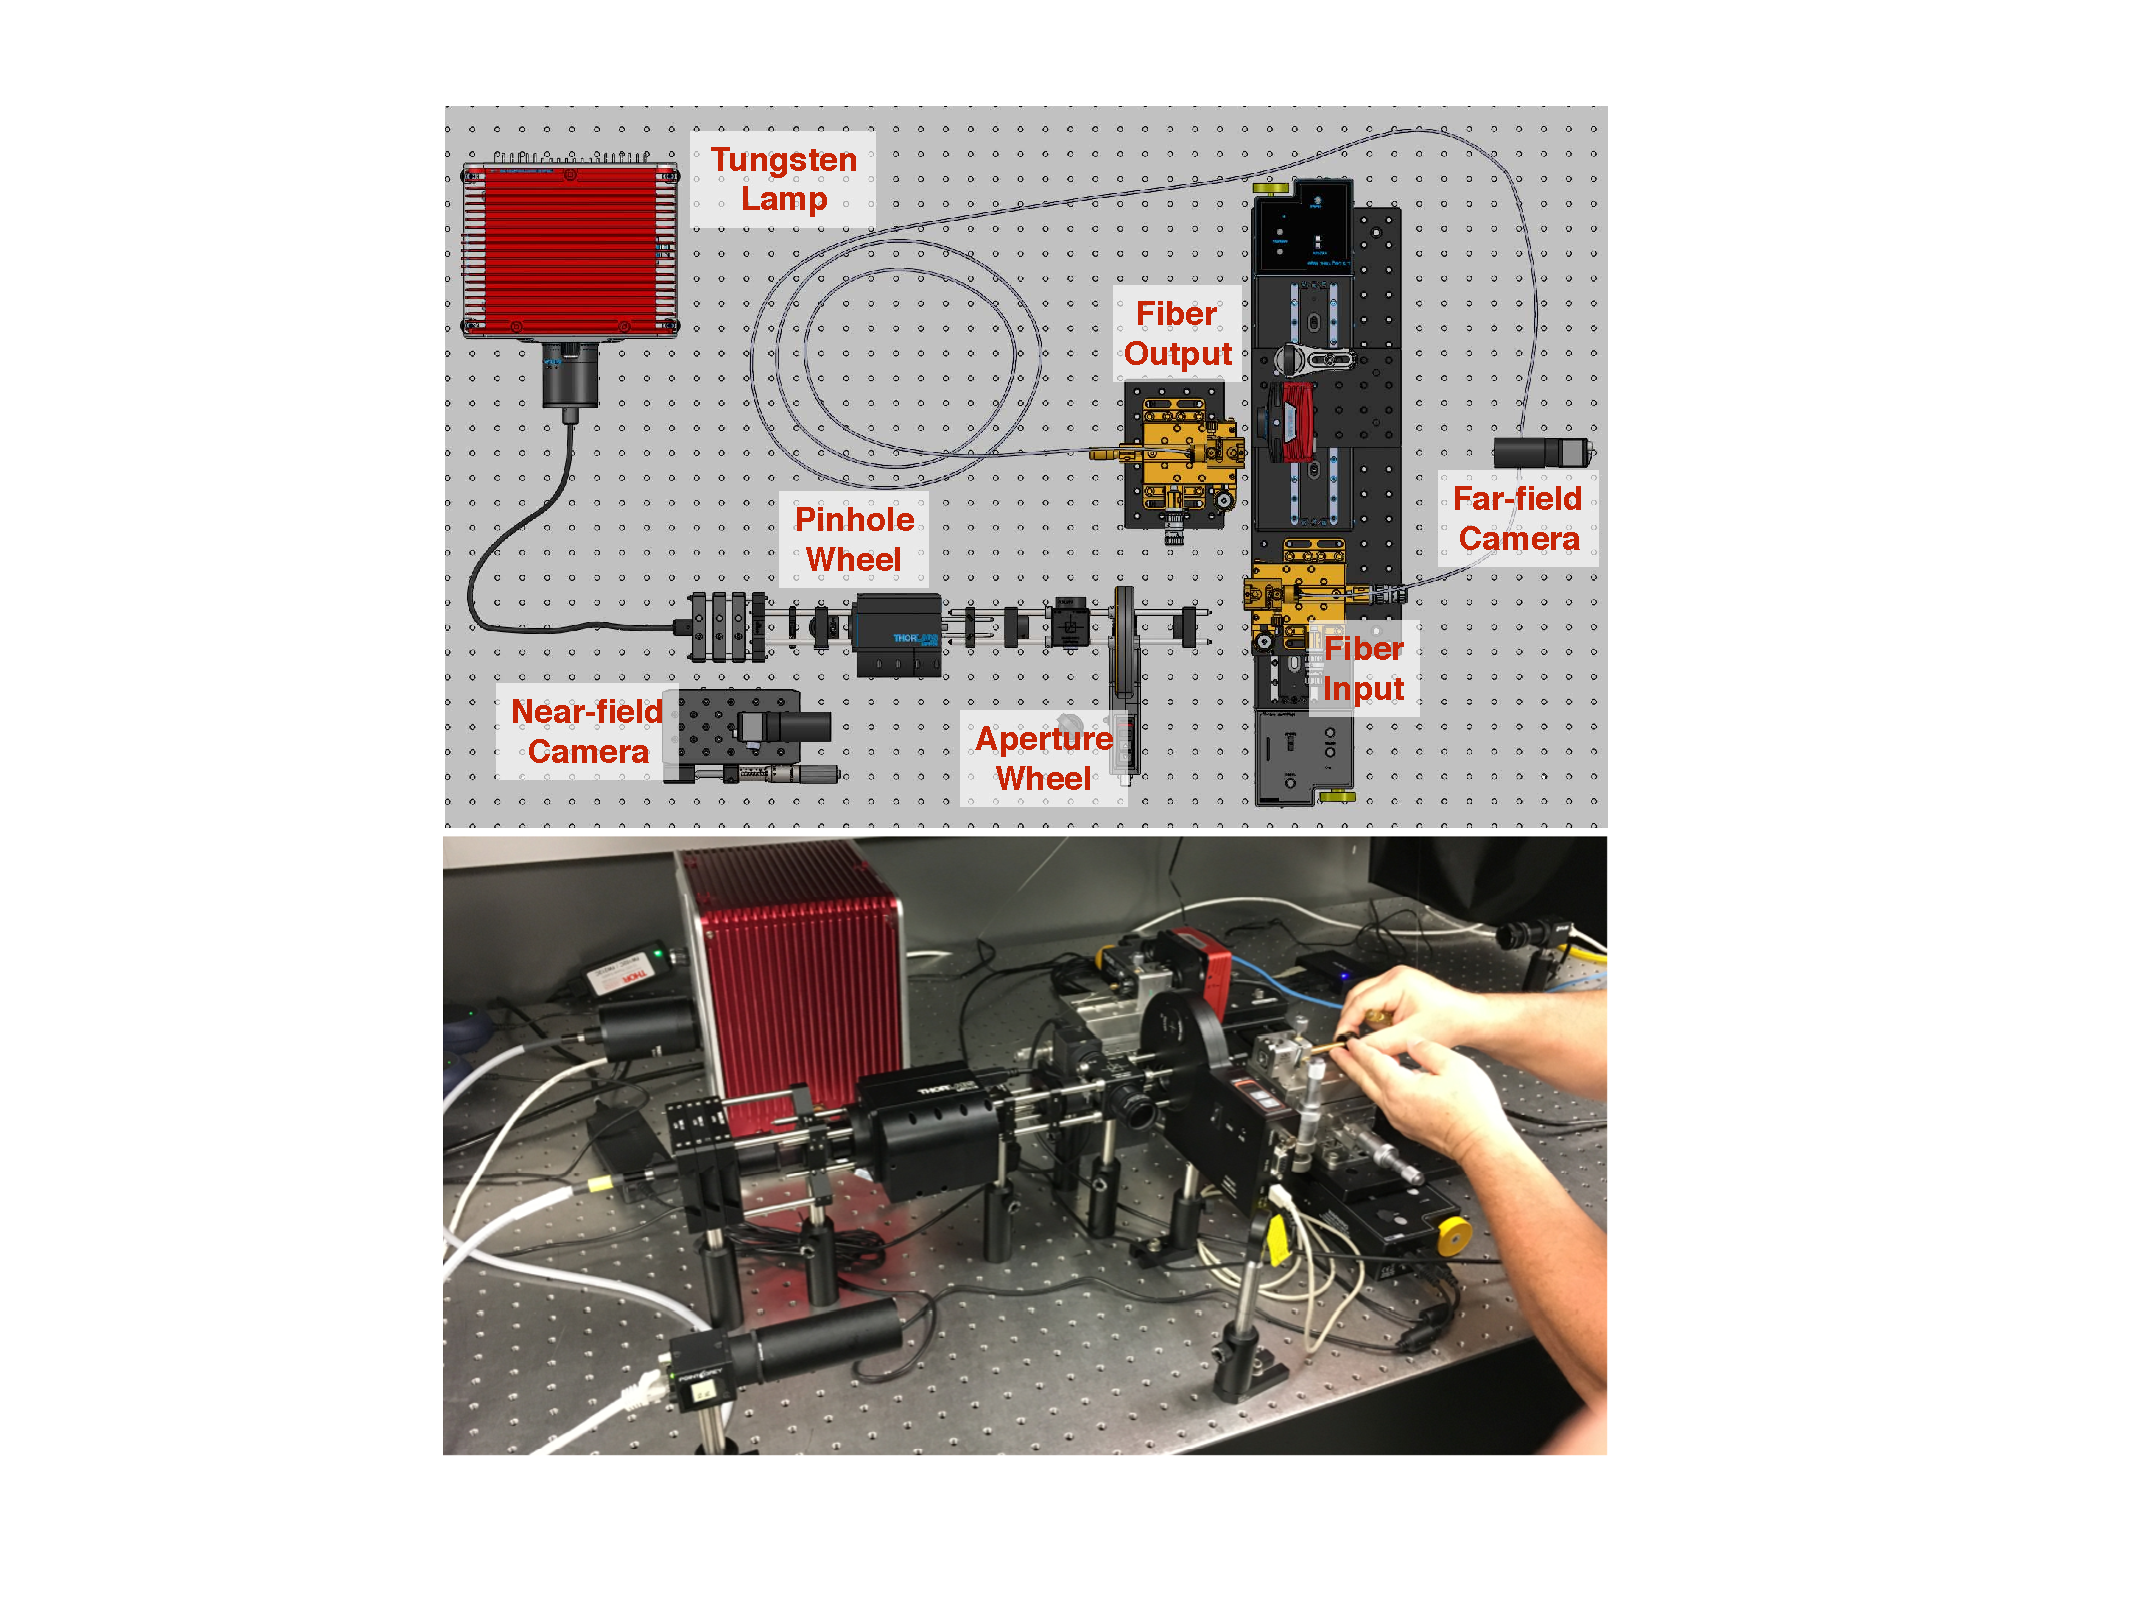
\includegraphics[width=0.9\textwidth]{figs/test_bench.pdf}
%figs/fig_test_bench.png}
%
\caption{\small  A schematic diagram (top) and photograph (bottom) of
the UCO Fiber Test Bench used to prototype fiber-lenslet coupling
options and ensure high-throughput coupling at the Keck focal plane.
The test bench allows allows for variable input broadband sources to be
directly compared to output near- and far-field images generated after
the input light passes through fiber assemblies.}
%
\label{fig:testbench}
%
\end{figure}


\subsection*{Senior Personnel}

Senior personnel on our project are PI Bundy, co-PI Westfall, Becker,
Capak, Coil, Cooper, Guhathakurta, Mandelbaum, Newman, O'Meara,
Prochaska, Rau, Rhodes, Rockosi, Rich, Schafer, Shapley, Siana, Weisz,
Williams, and Wilson.  Funds are budgeted to support PI Bundy and co-PI
Westfall; no support is requested for remaining personnel.  The roles of
all senior personnel are described in our Project Team Supplementary
Document and, where appropriate, in the outline of our Project
Execution Plan. 

\subsection*{University of California Observatories}

The University of California Observatories (UCO) manages a world-renown
facility on the University of California, Santa Cruz, campus for the
design, construction, and testing of astronomical instrumentation.  With
a staff of leading optical designers, engineers, and instrument
scientists, UCO has a long heritage of producing state-of-the-art
instrumentation, including many spectrometers (e.g., DEIMOS), as well as
controls software for the Lick and Keck Observatories.  The recent
delivery of K1DM3\footnote{K1DM3: Keck 1 Deployable Tertiary Mirror.}
illustrates the close relationship between WMKO and UCO, which allows us
to leverage detailed knowledge of the observatory structure, protocols,
interfaces, software and systems requirements, and instrument
deliverables.

\subsection*{UCO Fiber Test Bench}

UCO has recently built a precision fiber test bench (Figure
\ref{fig:testbench}), which is currently being used to prototype lenslet
coupling solutions and procedures needed for coupling FOBOS fibers to
the Keck II focal plane.  As such, the test bench will serve as a
valuable testing tool in the FOBOS preliminary design, especially for
measuring the impact of fiber stress and motion on focal-ratio
degradation and beam stability.

\subsection*{W.~M.~Keck Observatory}

WMKO has provided funding as well as technical guidance for initial
stages of FOBOS development and its interface to the observatory.  The
underside of the Keck II Nasmyth deck (Figure \ref{fig:nasmyth_mount})
has been identified as the mounting point for FOBOS spectrographs,
maintaining access space for other Keck instruments above.  Figure
\ref{fig:keck_exchange} shows how railings allow instrument components,
like the FOBOS focal-plane system, to wheel up to the Nasmyth port or to
wheel back in stow positions when not in use.

\begin{figure}[h!]
%
\vskip -0.1in
%
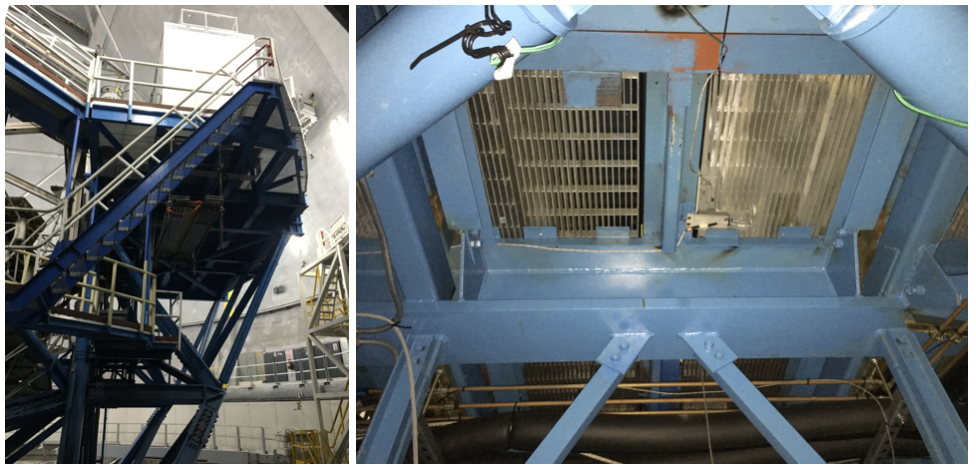
\includegraphics[width=\textwidth]{figs/nasmyth_deck.png}
%
\caption{\small The underside of the Keck II Nasmyth deck where the
FOBOS spectrographs will be mounted, with fibers fed from the
focal-plane system above.  Other Keck facility instruments (e.g.,
components of the adaptive optics laser system) have been successfully
mounted in this location.}
%
\label{fig:nasmyth_mount}
%
\end{figure}


\begin{figure}[h!]
%
\vskip -0.1in
%
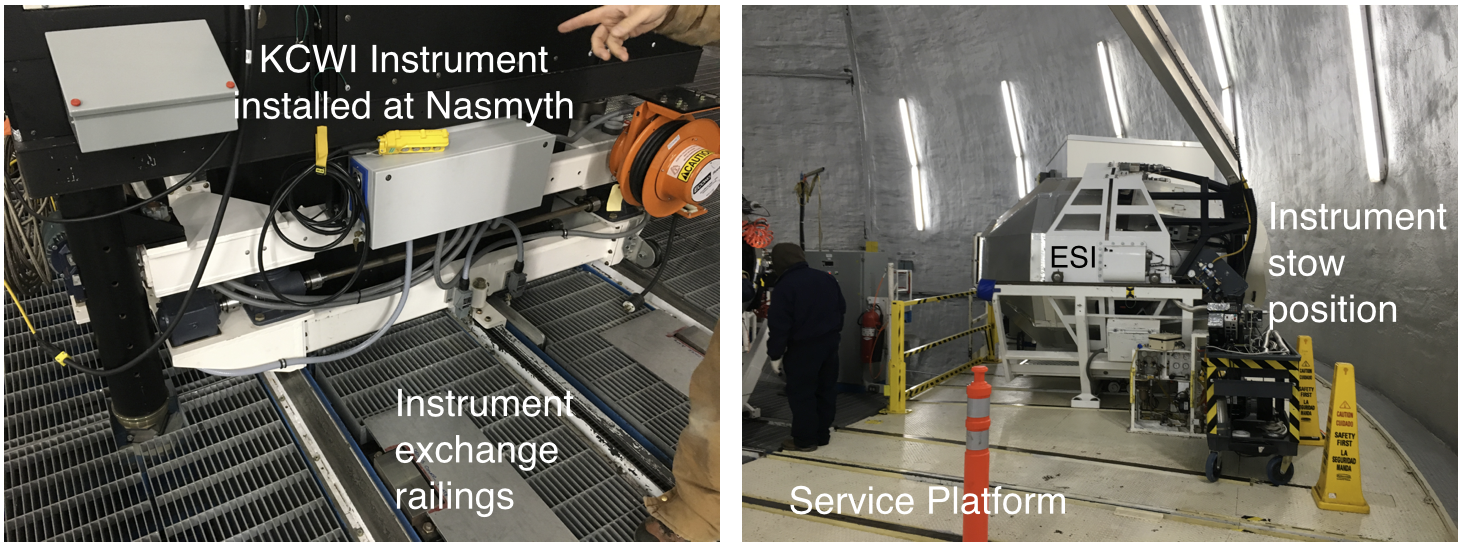
\includegraphics[width=\textwidth]{figs/Keck_instrument_exchange.png}
%
\caption{\small The FOBOS focal-plane system would be mounted on
railings to allow access to the Nasmyth port when its being used.  As
with other instruments, it can be removed to a stow position on the
extended service platform.  The photo on the left shows the Keck Cosmic
Web Imager (KCWI) in the Nasmyth mounted position.  On the right, the
Echellette Spectrograph and Imager (ESI) is shown in its stow position.}
%
\label{fig:keck_exchange}
%
\end{figure}

\subsection*{Starbugs at the Australian Astronomical Observatory}
\label{sec:AAO}

The Australian Astronomical Observatory (AAO) has worked with the FOBOS
team during conceptual design to develop designs for the CLADC and
confirm the feasibility of Starbugs at the FOBOS focal plane.  The
Starbugs fiber positioners have been under development at AAO for nearly
15 years \citep[see][]{staszak16} and have recently been deployed on-sky
on a new instrument called TAIPAN.  Beginning science operations this
year, TAIPAN demonstrates that the level of maturity attained by the
Starbugs technology makes it highly attractive to an instrument like
FOBOS beginning its preliminary design phase.

\begin{figure}[h!]
%
\vskip -0.1in
%
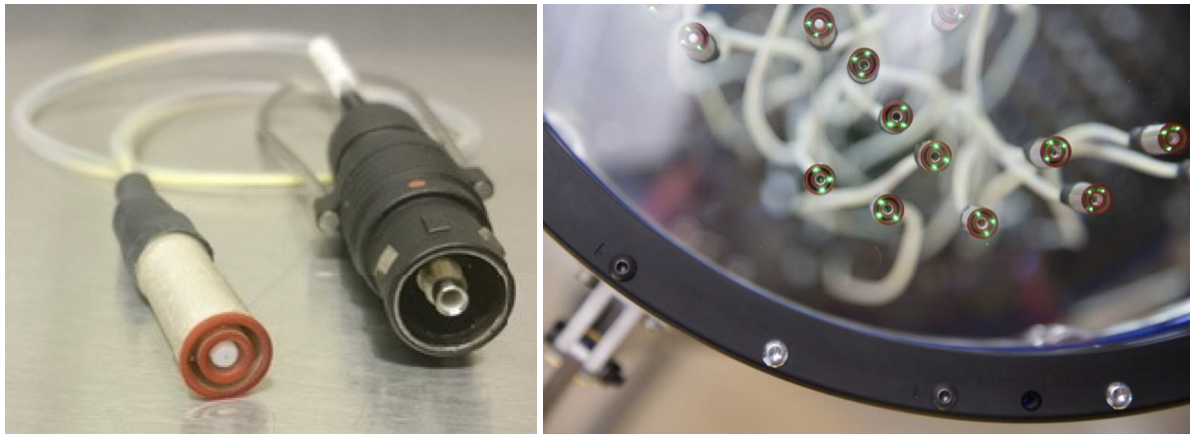
\includegraphics[width=\textwidth]{figs/starbugs.png}
%
\caption{\small Starbugs fiber positioning technology from AAO
\citep[from][]{staszak16}.  {\it Left:} An individual Starbug assembly
where the concentric piezo cylinders (colored red) that establish a
vacuum seal to the focal plane plate are evident with the central fiber
payload housing (white).  The outer diameter is 8mm.  A connector
directs the fiber output to the next section of the cable run. {\it
Right:} The picture shows the front face of several Starbugs attached to
the TAIPAN focal plane.  Three green laser dots provide closed-loop
feedback on each Starbug's position.}
%
\label{fig:starbugs}
%
\end{figure}

% Figure 7.  The reference is Lorente et al 2016  https://arxiv.org/pdf/1608.02645.pdf

\subsection*{FOBOS Conceptual Design}

FOBOS conceptual design work has proceeded in parallel with a
fiber-based, Nasmyth-mounted instrument concept for the Thirty Meter
Telescope (TMT) that shared many design elements in common.  A variety
of related documents and reports are being produced in support of this
effort:

\begin{itemize}
%
\item Science Case Requirements Document: A funded effort to gather
community feedback, science cases, and associated requirements has
yielded the design specifications for FOBOS.  A report will be issued in
summer 2019.
%
\item Draft manuscript detailing requirements and demonstrating
necessary performance based on existing instrumentation for faint-object
fiber spectroscopy on large-aperture telescopes.
%
\item Design specification documents and optical (Zemax) models for the
CLADC, lenslet fiber fore-optics, spectrograph layout, and cameras.
%
\item Vendor quote estimates for the CLADC, Starbugs positioners, fiber
run, dichroics, FSE gratings, catadioptric cameras, and detector
systems.
%
\item SolidWorks modeling of the focal-plane system is nearly finished
with spectrograph support and enclosure structures underway.  Likely
vendors of focal-plane motion systems identified.
%
\item Detailed Microsoft Project plans through Preliminary Design and
out to instrument deployment.  
%
\item Risk matrix capturing 48 risk items and scoring their probability
and consequence severity before and after mitigation strategies.
%
\end{itemize}

% NICK SAYS: 4.5 We have a solid conceptual design of what a FOBOS
% spectrograph would be as well.  I'd add that to the list.  Might be
% worth adding a zemax rendering of the spectrograph.  

\subsection*{CMU Machine Learning Department}

The Carnegie Mellon University Machine Learning department is one of the
leading institutes in the field of Machine Learning research.  Project
members Mandelbaum and Rau are long time collaborators of the CMU
Machine Learning department.  In particular, they collaborate closely
with Prof. Barnab{\'a}s P{\'o}czos, an internationally recognized expert
in the field of Bayesian Optimization and Machine Learning.  Our
data-science challenges will benefit from direct input from Mandelbaum,
Rau, and their collaborators with respect to survey optimization,
performed with the help of the readily available software package
Dragonfly\footnote{\url{https://github.com/dragonfly/dragonfly/}} that
was developed Prof. P{\'o}czos and his group.

% Include a blurb on the LSST ISSC ?

% subsection starbugs_at_the_australian_astronomical_obseravatory (end)

\bibliographystyle{nsf}
\bibliography{references}

\end{document}


